\section{利用简单图像组合图片}

这篇文章将介绍利用简单的数学计算进行图片的组合。
图 \ref{fig:rt1} 是处理的结果,将坦克世界中 IS-7 (\ref{fg:fn}) 坦克与地图 Karelia(\ref{fg:bg1}) 相融合。
\begin{figure}
    \centering
    \includegraphics[width=0.7\linewidth]{/img/compute-vision/basic-image-processing/combine-image/rt1.png}
    \label{fg:rt1}
    \caption{处理结果,版权属于 Wargaming.net}
\end{figure}
使用的原图是
\begin{figure}
    \centering
    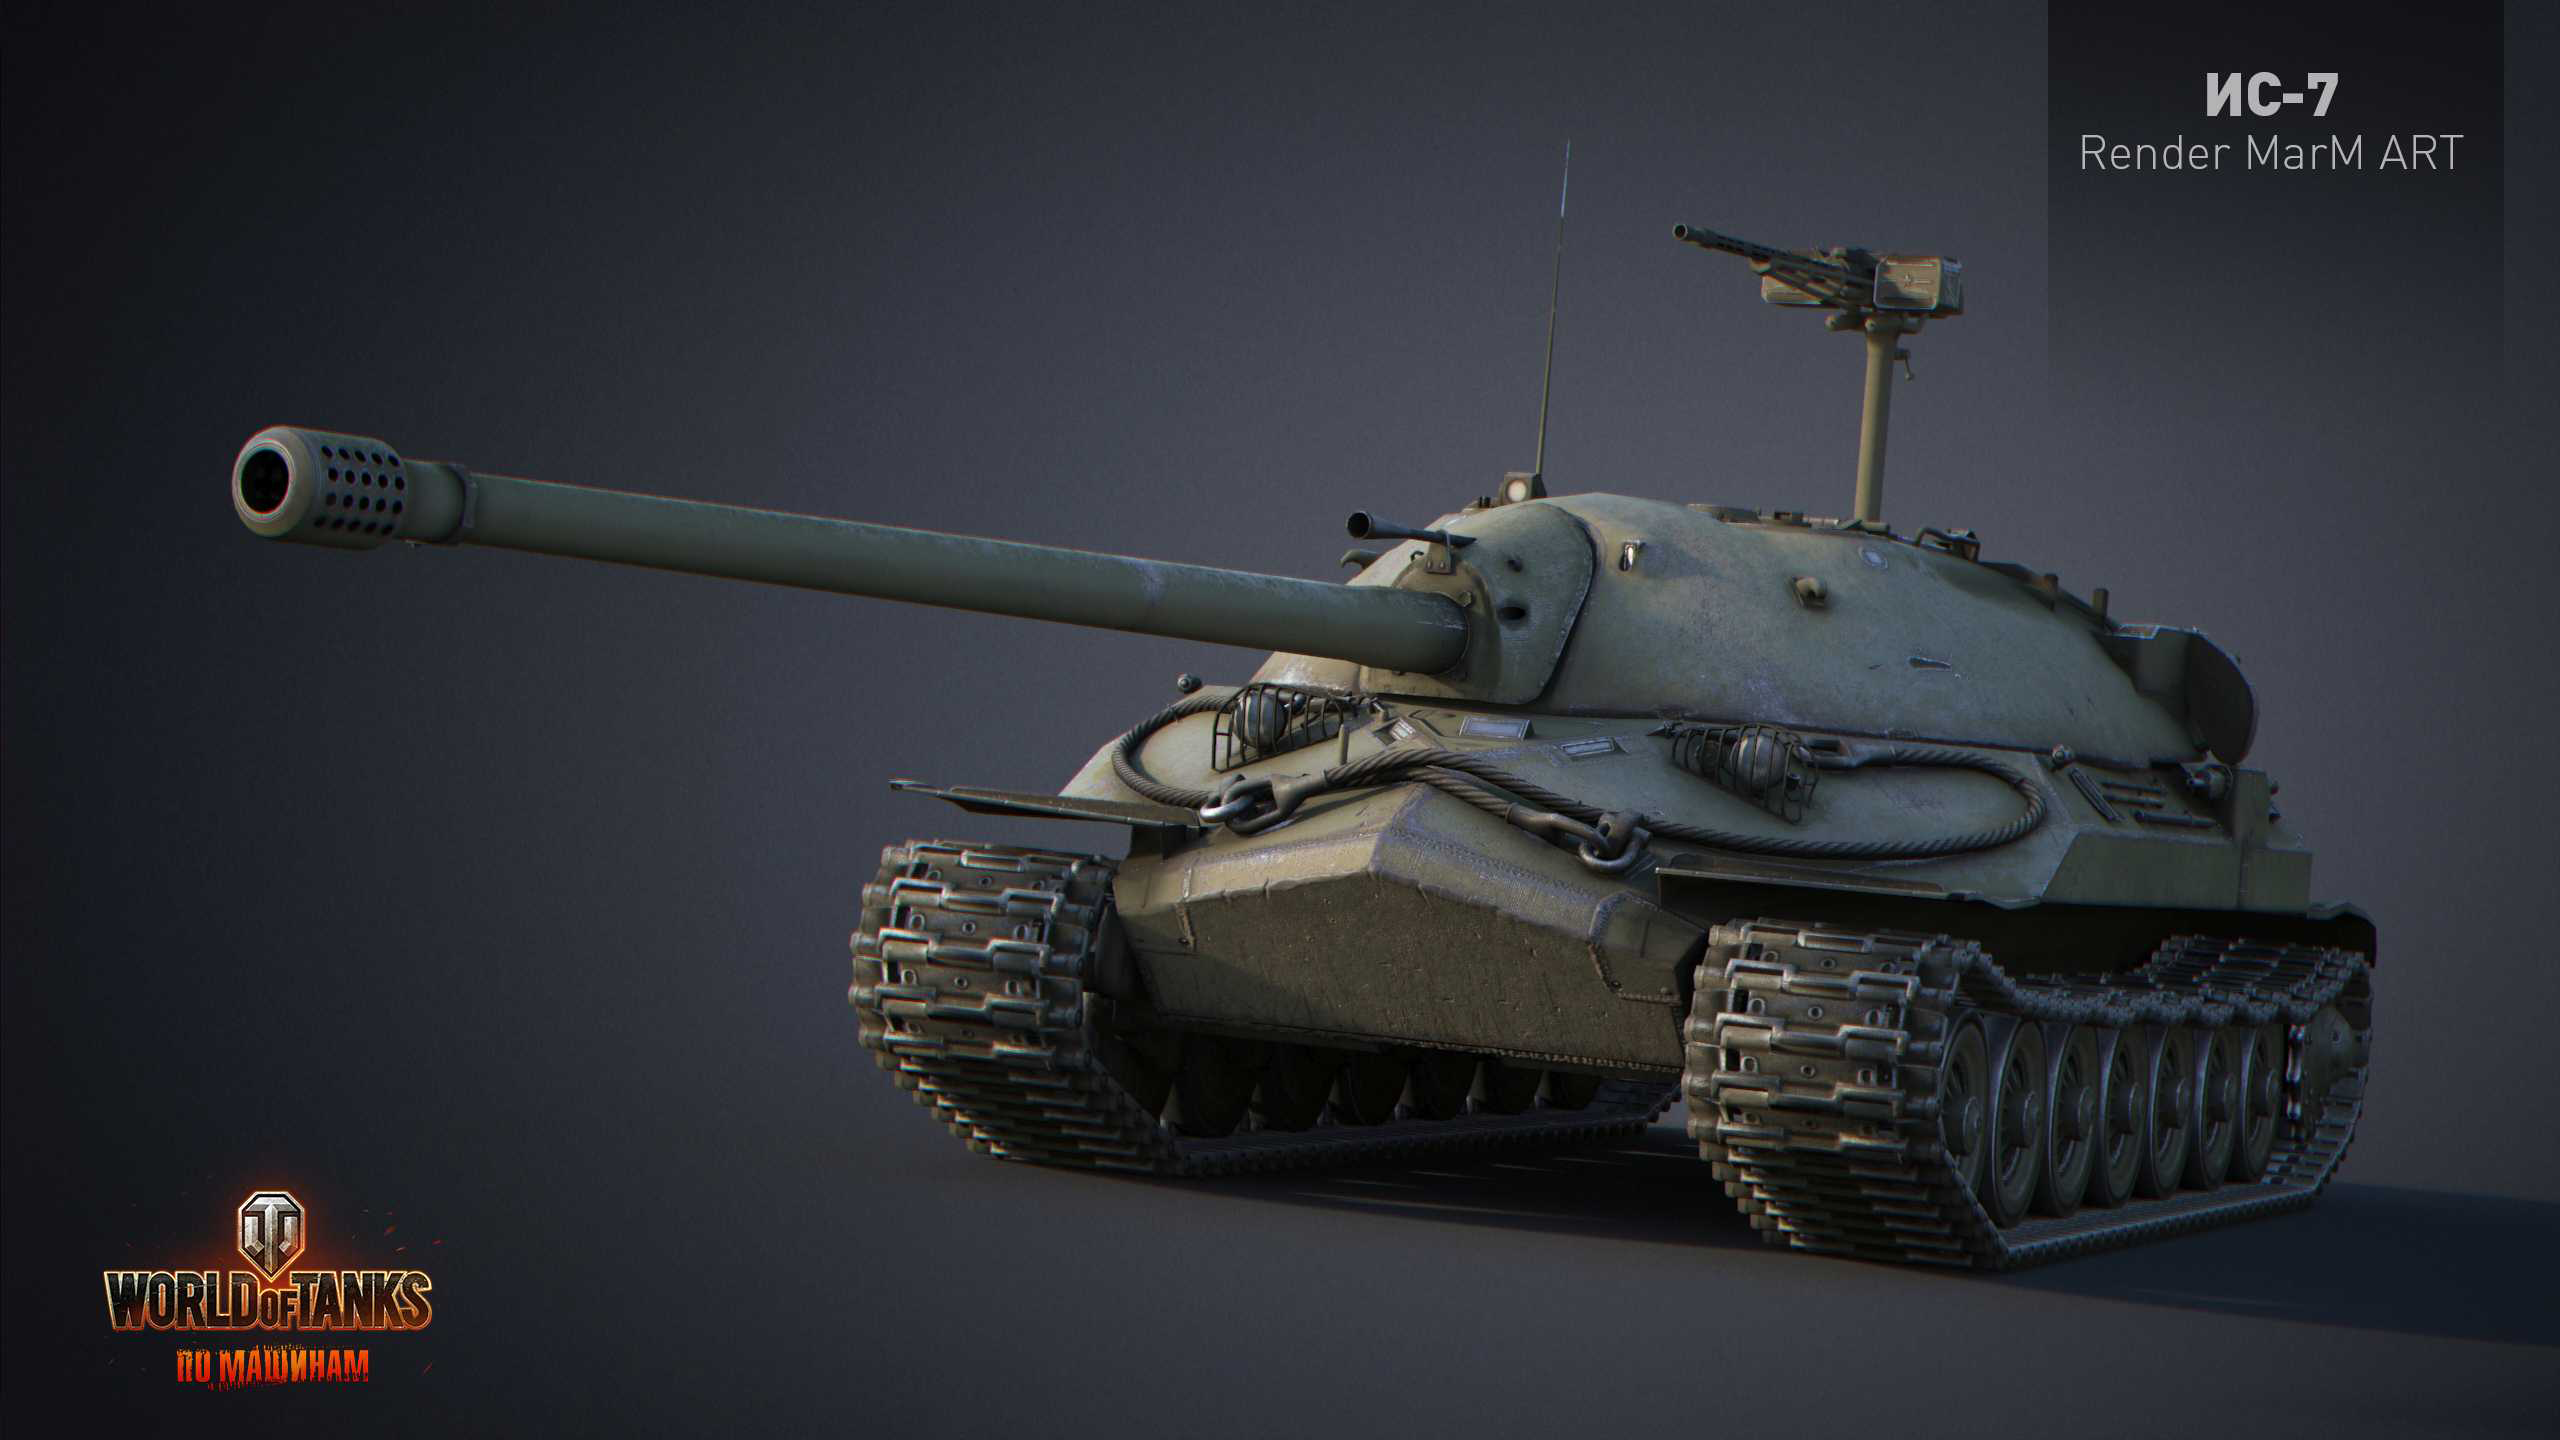
\includegraphics[width=0.7\linewidth]{/img/compute-vision/basic-image-processing/combine-image/fn1.png}
    \label{fg:fn}
    \caption{IS-7 坦克的图片,版权属于 Wargaming.net}
\end{figure}
\begin{figure}
    \centering
    \includegraphics[width=0.7\linewidth]{/img/compute-vision/basic-image-processing/combine-image/bg1.png}
    \label{fg:bg1}
    \caption{Karelia 地图的图片,版权属于 Wargaming.net}
\end{figure}

接下来将依次介绍数学理论与代码。

\subsection{数学基础}

\paragraph{线性组合}
第一个数学基础是线性组合。线性组合的公式如下
\[
    \mathbf{Z} = c_1 \mathbf{X} + c_2 \mathbf{Y}
\]
其中 $c_1$ 与 $c_2$ 分别是两个常量,然后 $\mathbf{X}$、$\mathbf{Y}$、$\mathbf{Z}$ 分别是三个矩阵。
实际上来说,$\mathbf{X}$、$\mathbf{Y}$、$\mathbf{Z}$ 也可以是向量或者高为矩阵。

如果将两幅图片的数据作为两个矩阵,则图 \ref{fg:lc} 是线性组合的结果。

\begin{figure}
    \centering
    \includegraphics[width=0.7\linewidth]{/img/compute-vision/basic-image-processing/combine-image/lc.png}
    \label{fg:lc}
    \caption{线性组合结果,权属于 Wargaming.net}
\end{figure}

\paragraph{线性组合进化版}
对于之前提到的线性组合,我们对  $c_1$ 与 $c_2$ 进行约束:
\[
    c_1 + c_2 = \alpha
\]
当我们取 $\alpha = 1$ 时,则有
\[
    \mathbf{Z} = c \mathbf{X} + (1 - c) \mathbf{Y}
\]
这个公式没有什么特殊的地方,唯一特殊在 $c$ 的取值,当 $c=1$ 的时候 矩阵 $\mathbf{Z}$ 与 $\mathbf{X}$ 是相等的,
而当 $c=0$ 的时候 矩阵 $\mathbf{Z}$ 与 $\mathbf{Y}$ 是相等的。
这一公式对于将两个图片的不同部分扣出然后组合在一起时有一定启发式的。

\paragraph{矩阵对应元素相乘:点乘}
线性组合中,标量 $c_1$ 与 $c_2$ 作用于整个矩阵。如果需要对矩阵中不同元素分别处理,
则需要将两个矩阵的元素对应相乘:
\[
    A \cdot B = \left( \begin{array}{cccc}
        a_{11} b_{11} & a_{12} b_{12} & \cdots & a_{1n} b_{1n} \\
        a_{21} b_{21} & a_{22} b_{22} & \cdots & a_{2n} b_{2n} \\
        \vdots          & \vdots          &        & \vdots          \\
        a_{m1} b_{m1} & a_{m2} b_{m2} & \cdots & a_{mn} b_{mn} \\
    \end{array} \right)
\]
这里暂将这个操作称作“点乘”。

\paragraph{线性组合:点乘升级版}
所以这里使用矩阵点乘升级一下线性组合:
\[
    \mathbf{Z} = \mathbf{C}_1 \cdot \mathbf{X} + \mathbf{C}_2 \cdot \mathbf{Y}
\]
其中  $\mathbf{X}$、$\mathbf{Y}$、$\mathbf{Z}$、$\mathbf{C}_1$、$\mathbf{C}_1$ 均为矩阵,
$\mathbf{C}_1$、$\mathbf{C}_1$ 可以被称作为参数矩阵。
进一步添加约束:
\[
    \mathbf{Z} = \mathbf{C} \cdot \mathbf{X} + (\mathbf(M) - \mathbf{C}) \cdot \mathbf{Y}
\]
其中 $\mathbf{M} = \{1\}_{m \times n}$ 是一个全 $1$ 矩阵。

本文最开始的图片\ref{fg:rt1}便是这个带有约束的矩阵点乘版的线性组合公式的应用。
图 \ref{fg:mask} 是使用的参数矩阵。
\begin{figure}
    \centering
    
\includegraphics[width=0.7\linewidth]{/img/compute-vision/basic-image-processing/combine-image/mask1.png}
    \label{fg:mask}
    \caption{利用的 Mask,权属于 Wargaming.net}
\end{figure}

\subsection{代码}
有了之前的数学基础,接下来就可以分析代码了。
一份\href{https://gist.github.com/Qinka/c118d6ab3e9f3d2a981ef6a1e84ac074}{代码} 是使用 CPU 运算的,
还有一份\href{https://gist.github.com/Qinka/d19cc950dc6b67e2e7a8d046bb9fa2cf}{代码}是使用 nVidia GPU 运算的。
代码使用我自己编写的 Haskell FAI 接口与一个简单的 BLAS 库完成的,在 \url{https://github.com/Qinka/HaskellFAI}
可以获取这代代码(你或许需要去开发分支看看)。

\paragraph{图片读入与预处理}
我自己写的轮子中是使用 Hackage 中的 \href{http://hackage.haskell.org/package/JuicyPixels}{JuicyPixels}
读入图片。此外还可以使用诸如 OpenCV 之类的内容读取图片。

在读取图片之后,最好进行数据的预处理,目标是把像素值归一化,这样运算就会简便不少。
例如使用八位 RGB 格式的图片,预处理就是先把 8位整数转换成浮点数,然后除以他们的最大值 $255$。

\paragraph{获取掩模}
如果你要问“掩模”是啥,我只能和你说,我给参数矩阵 $\mathbf{C_1}$ 与 $\mathbf{C_2}$ 起了一个外号。

我们需要将两张图片的部分进行组合,对于一个像素,要么来自于图片 X,要么来自于图片 Y。
则参数矩阵 $\mathbf{C_1}$ 与 $\mathbf{C_2}$ 是简单的二值矩阵,只包含 0或者1。
下面公式则能将图片合并
\[
    \mathbf{Z} = \mathbf{C} \cdot \mathbf{X} + (\mathbf(M) - \mathbf{C}) \cdot \mathbf{Y}
\]
其中 $\mathbf{M} = \{1\}_{m \times n}$ 是一个全 $1$ 矩阵。
而 $\mathbf{C}$ 是图 \ref{fg:mask} 对应的矩阵。
图 \ref{fg:mask} 是使用 Photoshop 手工抠出来的轮廓。当然也可以使用更高级的方法去抠。
Photoshop 抠出来的掩模保存成图片,之后处理图片是一并被读入。

\paragraph{实现}
实现的代码很简单,
\begin{lstlistings}[language=Haskell]
bufMB <- nForwardDotPrd bufM1 sn1 >>= nForwardAdd s1 >>= (`nForwardSub` bufM2)
cutP1 <- nForwardDotPrd bufPF bufM1
cutP2 <- nForwardDotPrd bufPB bufMB
fin <- nForwardAdd cutP1 cutP2
\end{lstlistings}
这四行代码依次计算 $M-C$ 矩阵,$C \cdot X$ 矩阵,$(M - C) \cdot Y$矩阵 与 $C \cdot X + (M - C) \cdot Y$ 矩阵。
最后获得的 \verb|fin| 则是最后处理好的函数。
